\documentclass{beamer}
\usepackage{amssymb}
\usepackage{amsmath}
\usepackage{stmaryrd}
\usepackage{graphicx}
\usepackage{isabelle}
\usepackage{isabellesym}

\usepackage{ctex}

%%%%%%%%%%%% For Isabelle code
\newlength{\fminilength}
\newsavebox{\fminibox}
\newenvironment{fmini}[1][\linewidth]
  {\setlength{\fminilength}{#1\fboxsep-2\fboxrule}%
   \vspace{2ex}\noindent\begin{lrbox}{\fminibox}\begin{minipage}{\fminilength}%
   \mbox{ }\hfill\vspace{-2.5ex}}%
  {\end{minipage}\end{lrbox}\vspace{1ex}\hspace{0ex}%
   \framebox{\usebox{\fminibox}}}

\newenvironment{specification}
{\noindent\scriptsize
\tt\begin{fmini}\begin{tabbing}X\=X12345\=XXXX\=XXXX\=XXXX\=XXXX\=XXXX
\=\+\kill} {\end{tabbing}\normalfont\end{fmini}}

\usetheme{Warsaw}
\def \twoSpaces {\ \ }

\def \oneSpace {\ }

\def \oneSpace {\ }
\def \eqc {= }
\def \andc {\wedge }
\def \negc {\neg }
\def \orc {\vee }

\begin{document}

%%-------------------------------------------------


\title{ {\sf paraVerifier}: An Automatic Framework for Proving Parameterized Cache Coherence Protocols}
%\titlerunning{{\sf paraVerifier}: An Automatic Framework for Proving Parameterized Cache Coherence Protocols}

\author{Yongjian Li\inst{1,3} \and Jun Pang\inst{2} \and Yi Lv\inst{1}
\and Dongrui Fan\inst{4} \and \\ Shen Cao\inst{1} \and Kaiqiang Duan\inst{1}}

%\authorrunning{Li et al.}

\institute{
State Key Laboratory of Computer Science, China \and
Computer Science and Communications, University of Luxembourg, Luxembourg \and
College of Information Engineering, Capital Normal University, Beijing, China \and
Institute of Computing Technology, Chinese Academy of Sciences, China
}
\frame{\titlepage}
%%-------------------------------------------------

\begin{frame}\frametitle{Problem of Parameterized Verification}
Consdier a protocol $P$, a property $Inv$
\begin{itemize}
\item  $P(N) \models Inv$ for any $N$
\item not just for a single protocol instance  $P(c)\models Inv$
\item Our opnion: a theorem proving problem becasue we cann't enumerate all protocol instance $P(N)$
\end{itemize}
\end{frame}

\begin{frame}\frametitle{State of Arts}
\begin{itemize}
\item CMP:  parameter abstraction and parameter abstraction
\item Proposed, by McMillan, elaborated by Chou, Mannava, and Park (CMP) , and formalized
by Krstic
\item construction of an abstract instance which can simulate any protocol instance
\item human provides auxiliary invariants (non-non-interference lemmas)
\end{itemize}
\end{frame}


\begin{frame}\frametitle{State of Arts }
\begin{itemize}
\item  invisible invariants,
\item  auxiliary invariants are computed from reachable state set in a finite protocol
instance $P(c)$
\item raw formula translated from BDD
\item  the reachable state set cann't be enumerated, e.g., the FLASH protocol
\end{itemize}
\end{frame}



\begin{frame}\frametitle{Two central and difficult problems}
\begin{itemize}
\item  searching auxilairy invariants is not automatical
\item  soundness problem: the theoretical foundation is not mechanized, and a gap between existing
approaches and a formal proof
\end{itemize}

\end{frame}

\begin{frame}\frametitle{Our Motivation}

\begin{itemize}
\item automatically searching  auxilairy invariants
\item Formally proving all the things: both the theoretical foundation and case studies
\item A formal proof script as a formal verification product
\end{itemize}
\end{frame}


\begin{frame}\frametitle{An Overview of Our Approach}


\begin{figure}[!t]
\centering %
\vspace{-0.8cm}
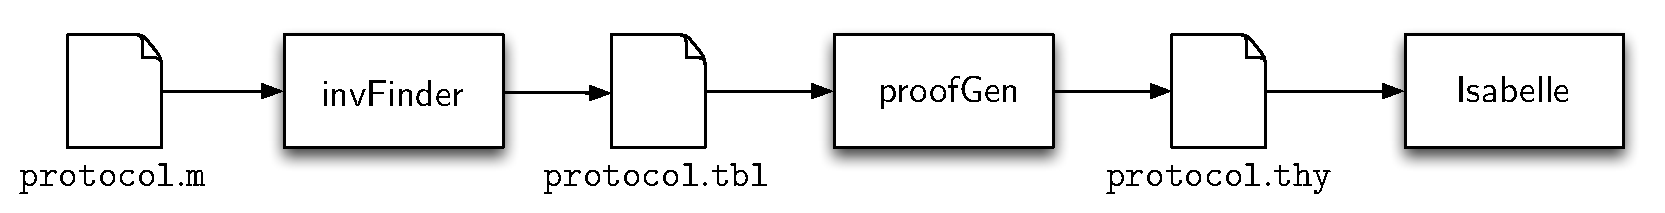
\includegraphics[width=1.0\textwidth]{paraVerifier.pdf}
\vspace{-0.6cm}
\caption{The workflow of {\sf paraVerifier}.}
\label{fig:arch}
\end{figure}
\end{frame}

\begin{frame}\frametitle{Some Explanations}

\begin{itemize}
\item {\sf paraVerifier}={\sf invFinder} + {\sf proofGen}

\item protoocl.fl: a small cache coherence protocol instance


\item {\sf invFinder} searches auxiliary invariants automatically
\item Some advanced theories: Kepler guess, Four-coloured problems

\item   protocol.tbl:  stores the set of ground invariants and a causal relation table

\item {\sf proofGen}: create an Isabelle proof script {\sf protocol.thy} which models and verifies the protocol

\item run Isabelle to automatically proof-check {\sf protocol.thy}
\end{itemize}

\end{frame}

\begin{frame}\frametitle{Theoretical Foundation-Protocol}
\noindent
A cache coherence protocol is formalized as a pair $({\it ini}, {\it rules})$, where
(1) ${\it ini}$ is an initialization formula; and
(2) ${\it rules}$ is a set of transition rules. Each rule $r\in {\it rules}$ is defined as
  $g \vartriangleright  S$, where $g$ is a predicate, and $S$ is a
  parallel assignment to distinct  variables $v_i$ with expressions
  $e_i$. We write $\mathsf{pre}~r=g$, and $\mathsf{act}~r=S$
  if $r=g \vartriangleright S$, where $S$ is  a parallel assignment $S=\{x_i:=e_i | i>0\}$.
\end{frame}

\begin{frame}\frametitle{An example-Mutual exclusion protocol}

\begin{specification}
 pini  N $\equiv$
   x=true $\wedge$  forallForm N ($\lambda$ i. n[i]=I))\\

    try i $\equiv$ n[i] $\eqc$ I $\vartriangleright$ n[i] := T; \\

    crit i $\equiv$ n[i] $\eqc$ T\& x = true $\vartriangleright$  n[i] := C || x := false;  ;\\

%
   exit i $\equiv$ n[i] $\eqc$ C $\vartriangleright$ n[i] := E; \\


   idle  i $\equiv$  n[i] $\eqc$ E $\vartriangleright$ n[i] := I ||  x := true;
  \\% \\
   prules N $\equiv$ \{r. ex1P N ($\lambda$ i. r=crit   i)~$\vee$~ex1P N ($\lambda$ i. r=exit
i)  $\vee$\\
 ex1P N ($\lambda$ i. r=idle i)~$\vee$ ex1P N ($\lambda$ i.r=try i)\}\\
%\\

mutualEx N$\equiv$ (pIni~N, prules~N)\\

mutualInv i j $\equiv$
  $\neg$ (n[i]$\eqc$ C $\andc$ n[j]$\eqc$ C)\\

\end{specification}
\end{frame}

%\begin{lemma}\label{consistentLemma}%[(Consistency lemma)]
For a protocol $( ini,  rules)$,
we use $\mathsf{reachableSet}~   ini~ rules$
to denote the set of reachable states of the protocol.
Given a set of invariants $ invs$,
we have
$[| \mathsf{consistent}~  invs ~ ini~  rules;
  s \in \mathsf{reachableSet}~  ini~rules|]\Longrightarrow
  \forall  inv \in invs. \mathsf{formEval}~ inv ~s$
%\end{lemma}
\end{frame}

\begin{frame}\frametitle{Theoretical Foundation-Causal Relation}
\begin{definition}
We define the following relations
\begin{enumerate}
\item $\mathsf{invHoldForRule_1} ~f ~r \equiv \mathsf{pre}~ r \longrightarrow \mathsf{preCond}~ f ~(\mathsf{act}~ r)$, where $\mathsf{preCond}~S~f=f[x_i:=e_i]$, which substitutes each
occurrence of $x_i$ by $e_i$;
\item $\mathsf{invHoldForRule_2}~ f~ r \equiv f = \mathsf{preCond}~ f~(\mathsf{act}~ r)$;
\item $\mathsf{invHoldForRule_3}~ f~ r ~F \equiv$  $\exists f' \in F$ s.t.
$(f' \wedge (\mathsf{pre}~ r)) \longrightarrow \mathsf{preCond} ~f ~(\mathsf{act}   ~r)$;
\item $\mathsf{invHoldForRule}~ f~ r ~F$ represents a disjunction of $\mathsf{invHoldForRule_1}$, $\mathsf{invHoldForRule_2}$
and $\mathsf{invHoldForRule_3}$.
%\item $\mathsf{invHoldForRule}~ f~ r ~F \equiv (\mathsf{invHoldForRule_1} ~f
%  ~r) \lor (\mathsf{invHoldForRule_2} ~f ~r) \lor (\mathsf{invHoldForRule_3}~ f~ r~F)$.
\end{enumerate}
\end{definition}
\end{frame}

\begin{frame}\frametitle{Theoretical Foundation - Consistency Relation)}


\begin{definition}
A consistency relation, i.e., $\mathsf{consistent}~ {\it invs} ~{\it ini}~ {\it rules}$,
that holds between a protocol $({\it ini}, {\it rules})$ and
a set of invariants ${\it invs}=\{inv_1,\ldots, inv_n\}$,  is defined as:
%
\begin{itemize}
\item For any invariant ${\it inv} \in {\it invs}$ and state $s$,
if ${\it ini}$ is
evaluated as true at state $s$
(i.e., $\mathsf{formEval}~{\it ini}~s={\it true}$), then ${\it inv}$ is also evaluated as true at the state $s$.

\item For any ${\it inv} \in {\it invs}$ and $r\in {\it rules}$,
$\mathsf{invHoldForRule}~{\it inv}~r~{\it invs}$.
\end{itemize}
\end{definition}


\end{frame}




\begin{frame}\frametitle{Theoretical Foundation - Consistent Lemma}

\begin{lemma}\label{consistentLemma}%[(Consistency lemma)]
For a protocol $( ini,  rules)$,
we use $\mathsf{reachableSet}~   ini~ rules$
to denote the set of reachable states of the protocol.
Given a set of invariants $ invs$,
we have
$[| \mathsf{consistent}~  invs ~ ini~  rules;
  s \in \mathsf{reachableSet}~  ini~rules|]\Longrightarrow
  \forall  inv \in invs. \mathsf{formEval}~ inv ~s$
\end{lemma}
\end{frame}



\begin{frame}\frametitle{Key Algorithm of {\sf invFinder}}
\begin{specification}
1\twoSpaces let findInvsFromRule  chk choose  tautChk isNew rule inv newInvs invs casRel=\\
%2\twoSpaces  let rule=ruleApp pRule paras in\\
2\twoSpaces   val (g $\vartriangleright$ S)=rule in\\

3\twoSpaces   let inv'=preCond S inv in\\


4\twoSpaces   if  inv=inv' then\\

5\twoSpaces  \twoSpaces       let relItem=(rule,
inv,invHoldForRule2~inv~r) in\\
6\twoSpaces  \twoSpaces         (newInvs, relItem:casRel)\\


7\twoSpaces   else if  tautChk (g $\longrightarrow$inv') then\\
8\twoSpaces  \twoSpaces     let relItem=(rule, inv, invHoldForRule1~inv~r) in \\
9\twoSpaces  \twoSpaces        (newInvs, relItem:casRel)   \\


10\oneSpace   else let  candidates= subsets (decompose ((dualNeg inv') $\andc$ g ))  in\\

11\twoSpaces  \twoSpaces  let newinv =  choose chk candidates in\\
%12\twoSpaces       val ($\neg$ andList [items])=inv' in\\
%13\twoSpaces       let newinv= $\neg$ (andList ([items]@(and2Ands ant) )) in\\


12\twoSpaces  \twoSpaces     let relItem=(rule, inv,  invHoldForRule3 inv newInv   ) in\\

13\twoSpaces  \twoSpaces   if   ((isNew newInv (newInvs@invs)) then\\
14\twoSpaces  \twoSpaces   (newInvs@[normalize newInv], relItem\#casRel)\\
15\twoSpaces  \twoSpaces   else (newInvs,  relItem\#casRel)\\


16\oneSpace  else  error ``no new invariant";\\
\end{specification}
 \end{frame}


\begin{frame}\frametitle{More on {\sf invFinder}}


\begin{itemize}
\item trying to construct a consistency relation that
guides the tool {\sf invFinder} to find auxiliary invariants

\item using an oracles that checks whether a ground
formula is an invariant in the small reference model


\item Searching not only auxiliary invariants but also causal relations

\item   protocol.tbl:  storing the searching result
\end{itemize}
 \end{frame}

\begin{frame}\frametitle{A fragment of protocol.tbl}
 \begin{table}[!t]
\centering \caption{A fragment of output of {\sf invFinder}}\label{label-ground-causal relation} % {\tt
%simpMutual.tbl}
\begin{tabular}{|c|c|c|c|c|  }
\hline
  rule& ruleParas&inv&causal relation &   f'  \\
\hline
  .. & ..&.. &..&.. \\

\hline
  crit  & [1]&mutualInv 1 2& invHoldForRule3 &invOnX$_1$~2 \\
\hline
  crit &[2]& mutualInv 1 2& invHoldForRule3 &invOnX$_1$~1  \\
\hline
  crit & [3]& mutualInv 1 2 & invHoldForRule2  & \\
\hline
  .. & ..&.. &..&.. \\

\hline
  crit  & [1]&invOnX$_1$ 1 & invHoldForRule1 &\_ \\
\hline
  crit &[2]& invOnX$_1$ 1 & invHoldForRule1 &\_  \\
\hline
\end{tabular}
\end{table}
\begin{itemize}
\item invariants and causal relations are in concrete form
\item we need parameterized form (or symbolic form)



\end{itemize}
\end{frame}


\begin{frame}\frametitle{ {\sf proofGen}}


\begin{itemize}
\item  generalizing a concrete index (formula or relation) into 
a symbolic one with constraints

\item generating an Isabelle proof script automatically 


\item generalization is abstraction in essence
\end{itemize}
 \end{frame}
 
\begin{frame}\frametitle{ {\sf The generated Isabelle proof script}}


\begin{itemize}
\item Formal definition of   invariants and all actual invariants  

\item Formal definition of   rules and all actual rules 


\item Lemmas for causal relation between parameterized rules and invariants

\item Definitions and lemmas on initial states

\item The main lemma and its proof

\end{itemize}
 \end{frame} 
 
 
\begin{frame}\frametitle{ A fragment of the proof script}
\begin{specification}
1lemma critVsinv1:\\
2  assumes  a1: $\exists$ \iR1. \iR1 $\le$ N $\wedge$ r=crit \iR1 and \\
  a2: $\exists$  \iInv1 \iInv2. \iInv1 $\le$ N $\wedge$ \iInv2 $\le$ N $\wedge$ \iInv1 $\neq$ \iInv2 $\wedge$ f=inv1  \iInv1 \iInv2\\
3  shows  invHoldForRule s f r (invariants
  N)\\
4  proof -\\
   from a1 obtain \iR1 where a1:\iR1 $\le$ N $\wedge$ r=crit \iR1 \\
   by blast\\
   from a2 obtain \iInv1 \iInv2 where \\
   a2: \iInv1 $\le$ N $\wedge$ \iInv2 $\le$ N $\wedge$ \iInv1 $\neq$ \iInv2 $\wedge$ f=inv1  \iInv1 \iInv2\\
   by blast \\
5  have iR1=\iInv1 $\vee$ \iR1=\iInv2 $\vee$ (\iR1 $\ne$ \iInv1 $\wedge$  \iR1 $\ne$ \iInv2) by auto\\

6  moreover\{assume  b1:\iR1=\iInv1\\
7  \twoSpaces have invHoldForRule3 s f r (invariants N)\\
 \twoSpaces  \twoSpaces   proof(cut\_tac a1 a2 b1, simp, rule\_tac x=$\negc$ (x=true $\andc$ n[\iInv2]=C)  in exI,auto)qed\\
8  \twoSpaces then have invHoldForRule s f r
(invariants
  N)
by auto\}\\

9  moreover\{assume  b1:iR1=\iInv2\\
10 \twoSpaces have invHoldForRule3 s f r (invariants N)\\
 \twoSpaces \twoSpaces   proof(cut\_tac a1 a2 b1, simp, rule\_tac x=$\negc$ (x=true $\andc$ n[\iInv1]=C  in exI,auto)qed\\
11 \twoSpaces then have invHoldForRule s f r (invariants
  N)
by auto\}\\

12   moreover\{assume  b1:(\iR1 $\ne$  \iInv1 $\wedge$   \iR1 $\ne$  \iInv2)\\
13 \twoSpaces have invHoldForRule2 s f r  \\
  \twoSpaces \twoSpaces  proof(cut\_tac a1 a2 b1,  auto) qed\\
14 \twoSpaces then have invHoldForRule s f r
(invariants
  N)
by auto\} \\

15ultimately show invHoldForRule s f r
(invariants N) by blast\\
16qed\\
\end{specification}

 \end{frame} 

\end{document}
